% begin module parametric-intro
\begin{frame}
\frametitle{Curves Defined by Parametric Equations}
\begin{columns}[c]
\column{.4\textwidth}

\psset{xunit=1cm, yunit=1cm}
\begin{pspicture}(-2.2, -0.5)(2.2,3.7)
\tiny
\fcAxesStandard{-2}{-0.5}{2}{3.5}
%Calculator input: plotCurve{}(\cos{}(t^{2}), t \sin{}t+\sin{}t, 0, 3)
\parametricplot[arrows=->, linecolor=\fcColorGraph, plotpoints=500] {0}{0.75}{t 2 exp 57.29578 mul cos t 57.29578 mul sin t 57.29578 mul sin t mul add }
\parametricplot[arrows=->, linecolor=\fcColorGraph, plotpoints=500] {0.75}{1.5}{t 2 exp 57.29578 mul cos t 57.29578 mul sin t 57.29578 mul sin t mul add }
\parametricplot[arrows=->, linecolor=\fcColorGraph, plotpoints=500] {1.5}{2.25}{t 2 exp 57.29578 mul cos t 57.29578 mul sin t 57.29578 mul sin t mul add }
\parametricplot[linecolor=\fcColorGraph, plotpoints=500] {2.25}{3}{t 2 exp 57.29578 mul cos t 57.29578 mul sin t 57.29578 mul sin t mul add }

\uncover<1>{\fcFullDot{0.987227}{ 0.545186} }
\uncover<2>{\fcFullDot{0.689498}{ 1.488321} }
\uncover<3>{\fcFullDot{-0.379452}{ 2.365079}}
\uncover<4>{\fcFullDot{-0.892288}{ 2.744270}}
\uncover<5->{\fcFullDot{0.866232}{ 2.296575} }
\uncover<6->{
\rput[l](0.89,2.396575){$\begin{array}{l}(x,y)\uncover<7->{= (f(t), g(t))} \\\phantom{(x,y)}\uncover<8->{=(x(t), y(t))}\end{array}$}
}
\end{pspicture}
%\ \only<handout:0| -1>{%
%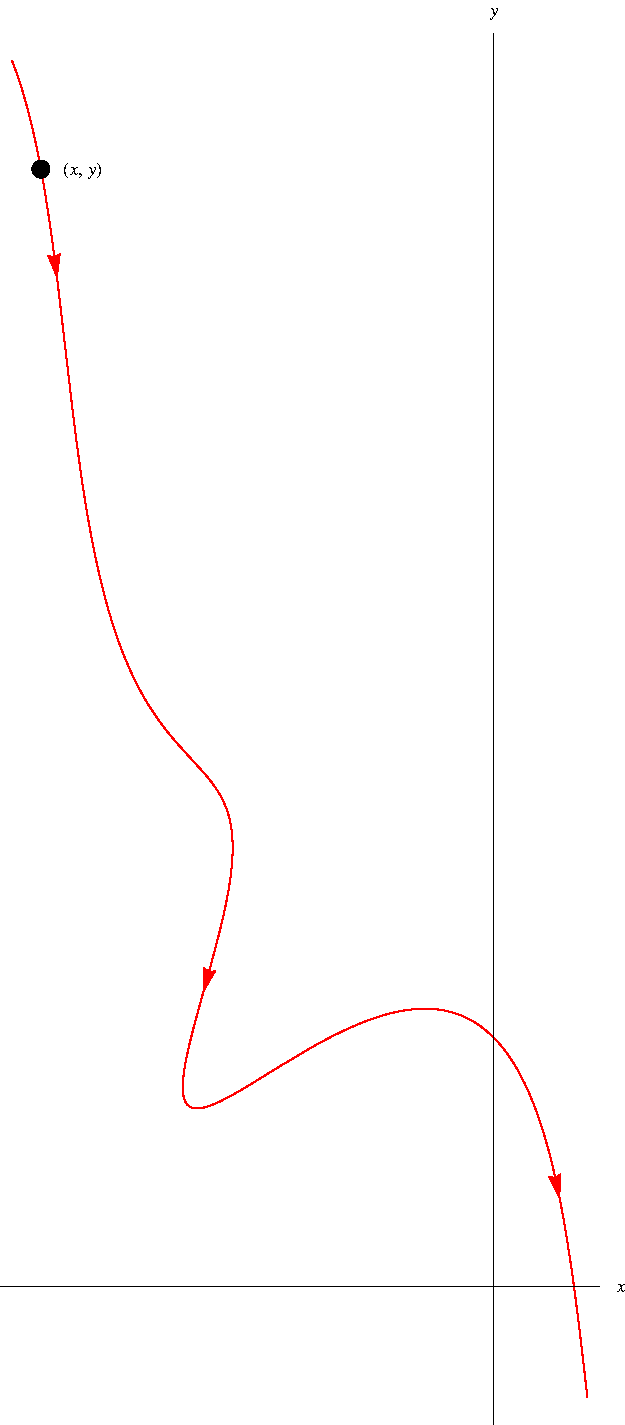
\includegraphics[height=7cm]{parametric-curves/pictures/11-01-parametrica.pdf}%
%}%
%\only<handout:0| 2>{%
%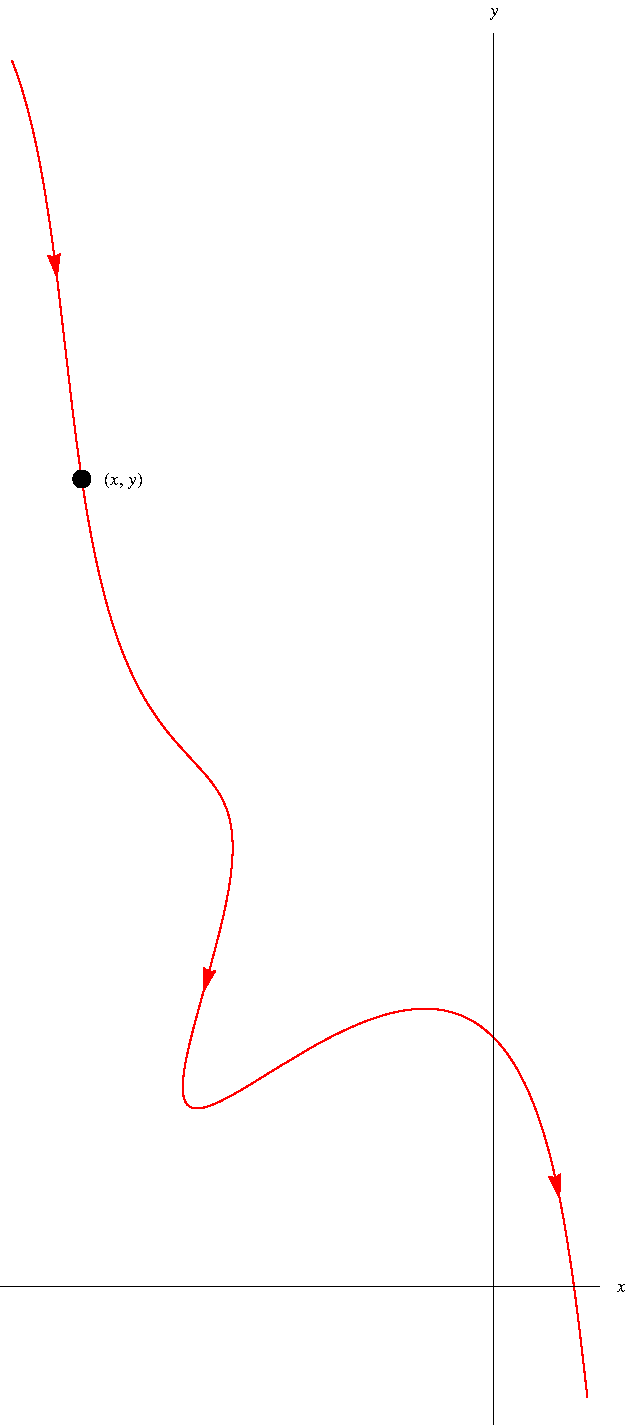
\includegraphics[height=7cm]{parametric-curves/pictures/11-01-parametricb.pdf}%
%}%
%\only<handout:0| 3>{%
%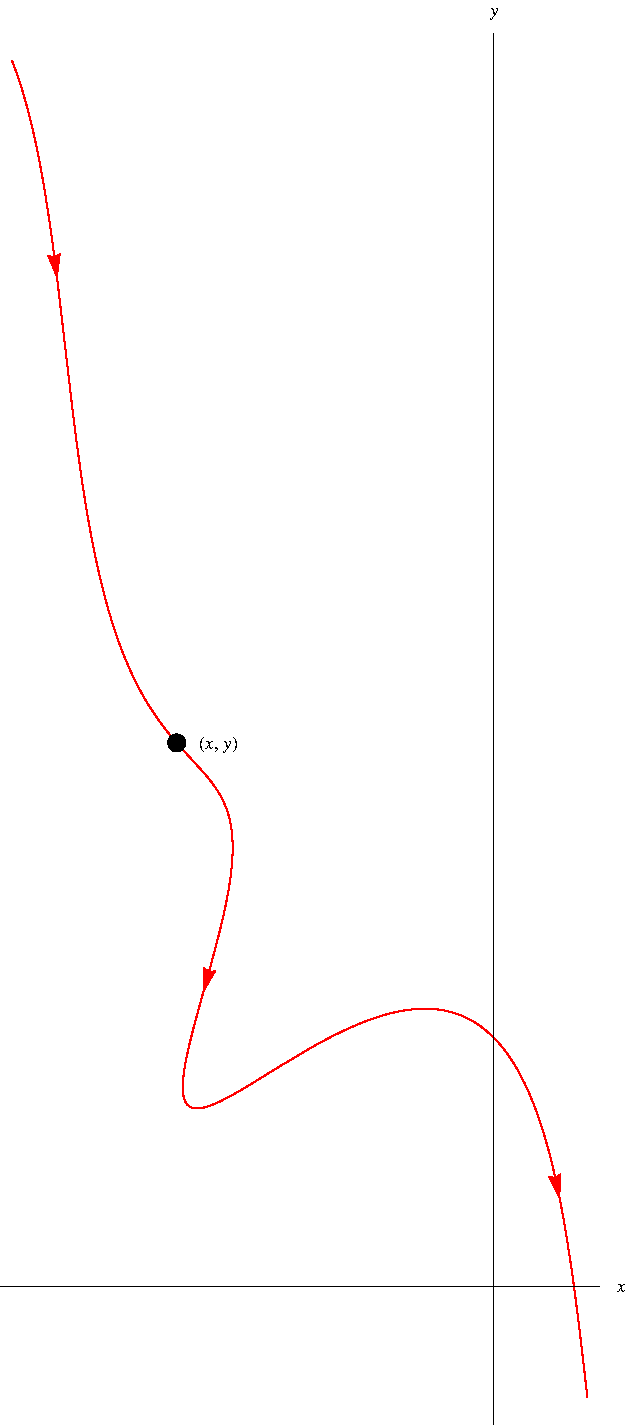
\includegraphics[height=7cm]{parametric-curves/pictures/11-01-parametricc.pdf}%
%}%
%\only<handout:0| 4>{%
%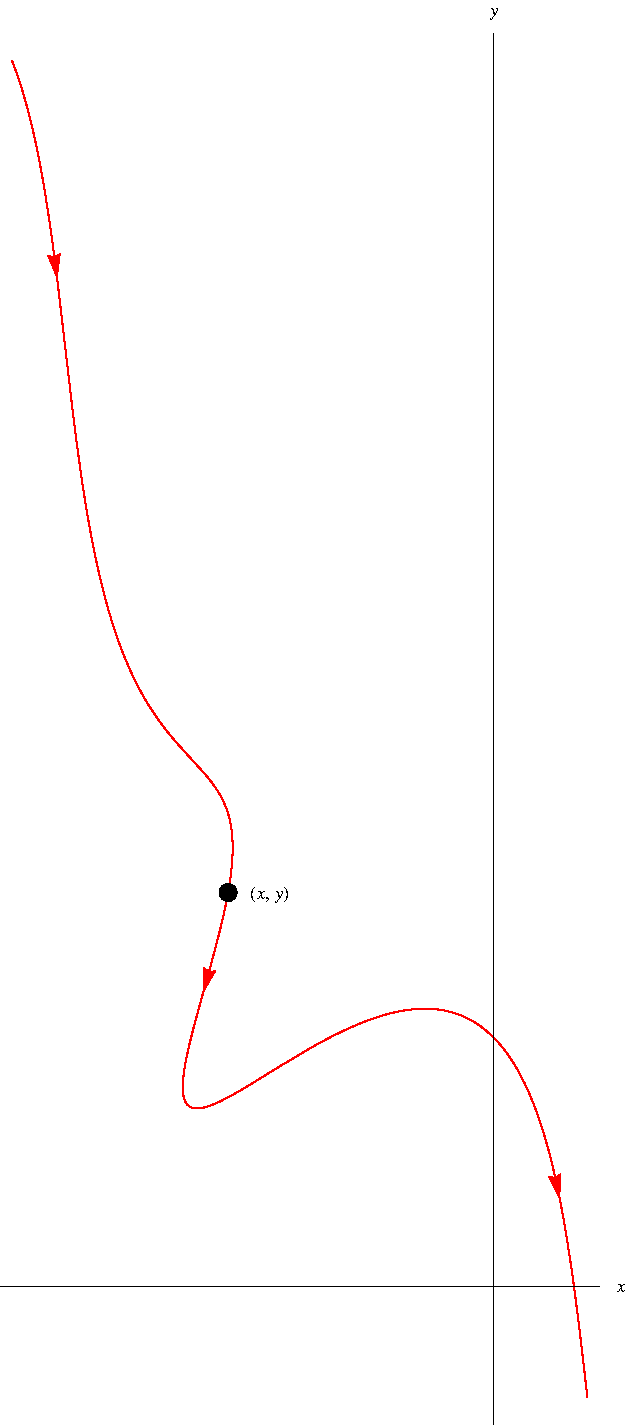
\includegraphics[height=7cm]{parametric-curves/pictures/11-01-parametricd.pdf}%
%}%
%\only<handout:0| 5-7>{%
%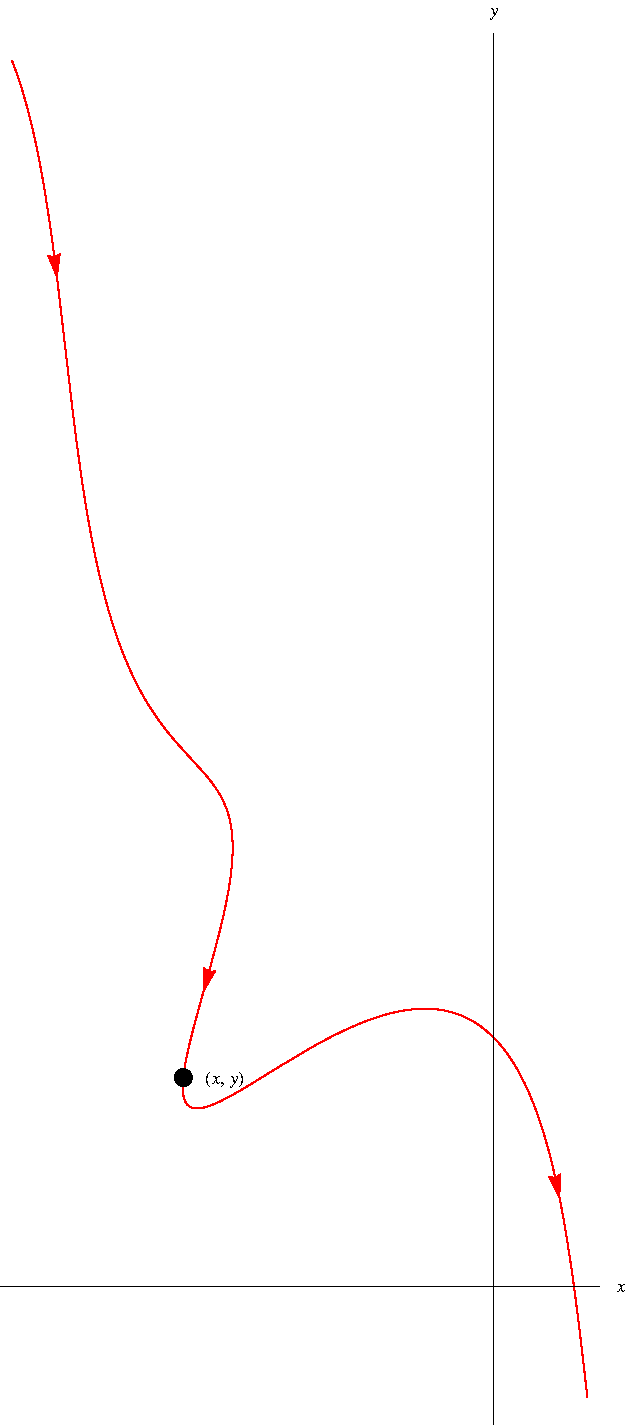
\includegraphics[height=7cm]{parametric-curves/pictures/11-01-parametrice.pdf}%
%}%
%\only<8->{%
%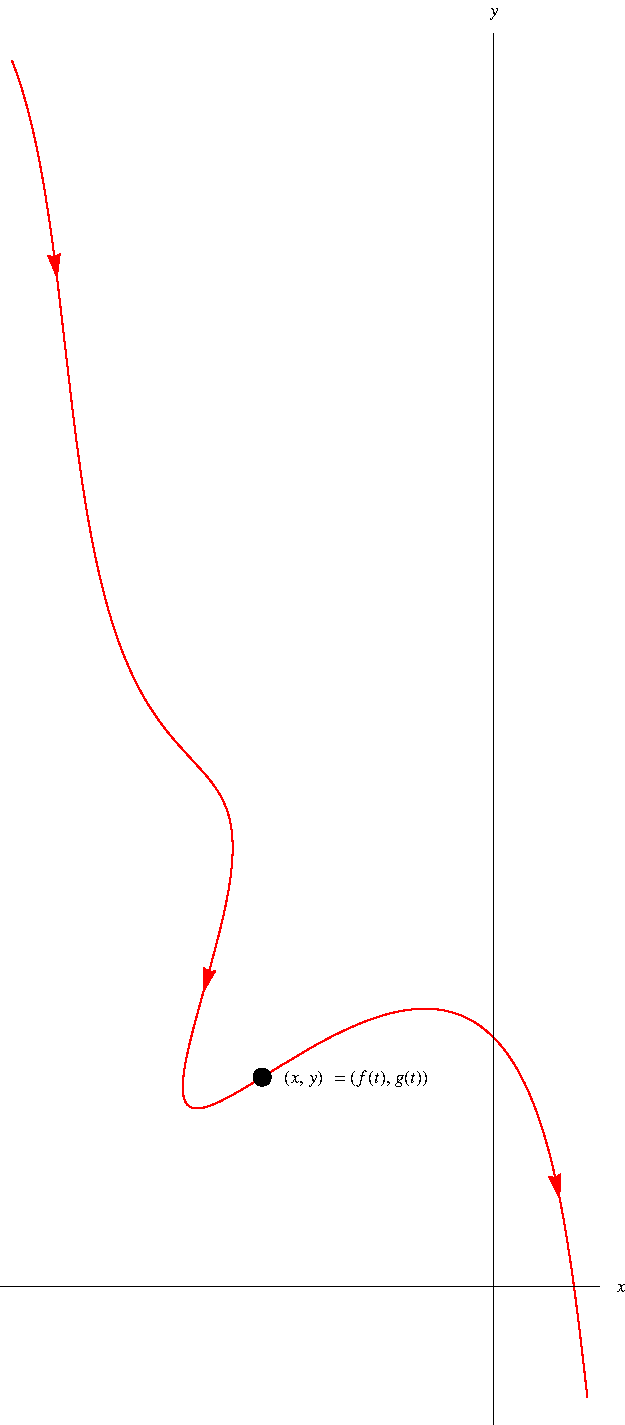
\includegraphics[height=4cm]{parametric-curves/pictures/11-01-parametricf.pdf}%
%}%
\column{.6\textwidth}
\begin{itemize}
\item  Suppose a particle moves along the curve in the picture.
\item<6->  The $x$-coordinate and $y$-coordinate of the particle are some functions of the time $t$.
\item<7->  We can write $x = f(t)$ and $y = g(t)$.
\item<8->  Less formally, we may directly write $(x,y)=(x(t), y(t))$.
\item<9->  We say that the equations $\left| \begin{array}{rcl}x &=& f(t)\\y&=&g(t)\end{array}\right.$ are parametric equations of a parametric curve.
\item<9->  Note that the curve can't be written as $y = f(x)$: it fails the vertical line test.
\end{itemize}
\end{columns}
\end{frame}
% end module parametric-intro
